\documentclass[a4paper]{article}
\usepackage[UTF8]{ctex}
\usepackage{geometry}
\usepackage{graphicx}
\usepackage{url}
\usepackage{multirow}
\usepackage{array}
\usepackage{booktabs}
\usepackage{url}
\usepackage{enumitem}
\usepackage{graphicx}
\usepackage{float}
\usepackage{amssymb}
\usepackage{amsmath}
\usepackage{subfig}
\usepackage{longtable}
\usepackage{pifont}
\usepackage{color}

\allowdisplaybreaks

\geometry{a4paper, scale=0.78}

% \begin{figure}[H]
%     \centering
%     \includegraphics[width=.55\textwidth]{E.png}
%     \caption{矩阵与列向量的乘法}
%     \label{fig:my_label_1}
% \end{figure}

% \left\{
% \begin{array}{ll}
%       x+2x+z=2 & \\
%       3x+8y+z=12 & \\
%       4y+z=2
% \end{array}
% \right.

% \begin{enumerate}[itemindent = 1em, itemsep = 0.4pt, parsep=0.5pt, topsep = 0.5pt]

% \end{enumerate}

%\stackrel{a}{\longrightarrow}

%\underbrace{}_{} %下括号

%\tableofcontents %目录,并且目录页不记录页码
% \tableofcontents
% \newpage
% \setcounter{page}{1} %new page
% \clearpage

\title{Kalman Filter 02 Model Construction \& Solution}
\author{Chen Gong}
\date{17 January 2020}

\begin{document}
\maketitle
Filtering问题公式话的表达即为$P(z_t|x_1,x_2,\cdots,x_t)$,是一种On-Line Learning的思路,随着越来越多的数据不断的被观测到,隐藏状态得到不断的更新。也就是在观察变量序列$\{x_1,x_2,\cdots,x_t\}$下,求得隐变量状态$z_t$的分布。模型表达为如下所示:
\begin{figure}[H]
    \centering
    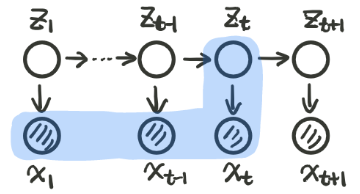
\includegraphics[width=.4\textwidth]{微信图片_20200116123639.png}
    \caption{模型基本拓扑结构}
    \label{fig:my_label_1}
\end{figure}

首先我们回顾一下前向算法的求解思路。在这个算法中首先定义了中间变量为:
\begin{equation}
    \alpha_t(i) = P(x_1,x_2,\cdots,x_t,z_t=q_i)
\end{equation}
而我们下一步则是要寻找$\alpha_{t+1}(i)$和$\alpha_t(i)$之间的关系。所以,可以按$\alpha_{1}(i),\alpha_{2}(i),\cdots,\alpha_{t}(i)$的顺序依次推断得到$\alpha_{t}(i)$,从而得到根据当前的模型推断出观测序列的分布$P(O|\lambda)$。

\section{Filtering问题思路}
我们还是采用的前向算法的思路:
\begin{equation}
    \begin{split}
        P(z_t|x_1,x_2,\cdots,x_t) 
        = & \frac{P(z_t,x_1,x_2,\cdots,x_t)}{P(x_1,x_2,\cdots,x_t)}  \\
        \propto & P(z_t,x_1,x_2,\cdots,x_t) \\
        = & \underbrace{P(x_t|x_1,x_2,\cdots,x_{t-1},z_t)}_{P(x_t|z_t)}P(x_1,x_2,\cdots,x_{t-1},z_t) \\
        = & P(x_t|z_t)\underbrace{P(z_t|x_1,x_2,\cdots,x_{t-1})}_{prediction}\underbrace{P(x_1,x_2,\cdots,x_{t-1})}_{const} \\
        \propto & P(x_t|z_t)P(z_t|x_1,x_2,\cdots,x_{t-1})
    \end{split}
\end{equation}

很显然通过如上的推导,我们将Filtering问题回归到了一个Prediction的问题。那么这个Prediction的问题,如何进一步求解呢?下一步,我们对Prediction的部分进行推导。
\begin{equation}
    \begin{split}
        P(z_t|x_1,x_2,\cdots,x_{t-1}) 
        = & \int_{z_{t-1}} P(z_t,z_{t-1}|x_1,x_2,\cdots,x_{t-1}) dz_{t-1} \\
        = &  \int_{z_{t-1}} \underbrace{P(z_t|z_{t-1},x_1,x_2,\cdots,x_{t-1})}_{P(z_t|z_{t-1})} \underbrace{P(z_{t-1}|x_1,x_2,\cdots,x_{t-1})}_{Filtering} dz_{t-1} 
    \end{split}
\end{equation}

通知上述的推导,我们又回到了一个Filtering的问题,那么这样我们形成了 一个递归的表达。那么,我们可以总结为在一个Filtering问题中,我们通过一个Prediction问题,来构建形成了一个回归。那么,下面我将详细的说明一下求解的过程:
\begin{equation}
    \begin{split}
        & t=1 \quad 
        \left\{
            \begin{array}{ll}
            P(z_1|x_1) & update \\
            p(z_2|x_1) & prediction \\
            \end{array}
        \right. \\
        & t=2 \quad 
        \left\{
            \begin{array}{ll}
            P(z_2|x_1,x_2) & update \\
            p(z_3|x_1,x_2) & prediction \\
            \end{array}
        \right. \\
        & \cdots\ \cdots \\
        & t=T \quad 
        \left\{
            \begin{array}{ll}
            P(z_T|x_1,x_2,\cdots,x_T) & update \\
            p(z_{T+1}|x_1,x_2,\cdots,x_{T-1}) & prediction \\
            \end{array}
        \right. \\
    \end{split}
\end{equation}

很显然,我们可以不断的往里面添加数据来更新隐变量状态$z_{t}$。

\section{Filtering问题求解具体分析}
首先,我们需要明确一个问题,Gaussian Distribution是一个具有非常好的性质的{\color{red}自共轭分布}。通俗的讲就是,Gaussian分布的边缘分布,条件分布,联合概率分布等都是符合高斯分布的。首位,我先回忆一下在Math Basis那小节中,总结的线性高斯模型中,已知条件高斯分布,求变量高斯分布的公式:
\begin{align}
    & P(X) = \mathcal{N}(X|\mu,\Lambda^{-1}) \\
    & P(Y|X) = \mathcal{N}(X|AX+b,L^{-1}) \\
    & P(Y) = \mathcal{N}(Y|AX+b,L^{-1}+A^{-1}\Lambda A) \\
    & P(X|Y) = \mathcal{N}(\Sigma\{ A^TL(y-b)+\Lambda\mu \}, \Sigma) \quad \Sigma = (\Lambda + A^TLA)^{-1}
\end{align}

从上小节中我们分析了Filtering问题的推导过程,我们可以看到Filtering问题可以被大致分成两个部分,也就是Prediction和Update两个部分。上一小节中我描述了大致的求解思路,那么这一小节我们将详细的描述怎么计算。

\subsection{Prediction}
预测问题被我们描述为,$P(z_t|x_1,x_2,\cdots,x_{t-1})$,那下面我们来进行分析怎么求。
\begin{equation}
    P(z_t|x_1,x_2,\cdots,x_{t-1}) = \int_{z_{t-1}} P(z_t|z_{t-1}) P(z_{t-1}|x_1,x_2,\cdots,x_{t-1}) dz_{t-1}
\end{equation}

根据Gaussian Distribution的自共轭性,所以$P(z_t|x_1,x_2,\cdots,x_{t-1})$一定是一个Gaussian Distribution。事实上$x_1,x_2,\cdots,x_{t-1}$中所有的信息都是已知的。为了方便表达$P(z_t|x_1,x_2,\cdots,x_{t-1}) \sim P(z_t)$。

那么,第$t-1$时刻的假设$P(z_{t-1}|x_1,x_2,\cdots,x_{t-1}) \sim \mathcal{N}(\mu_{t-1},\Sigma_{t-1})$。那么,第$t$时刻的分布$P(z_{t}|x_1,x_2,\cdots,x_{t}) \sim \mathcal{N}(\mu_{t}^\ast,\Sigma_{t}^\ast)$。并且,根据Gaussian Distribution的自共轭性,我们可以令$P(z_t|z_{t-1})\sim \mathcal{N}(z_t|Az_{t-1}+B,Q)$。令$x=z_{t-1},y=z_{t}$,代公式(5)-(7),可以计算出:
\begin{equation}
    \left\{
    \begin{array}{ll}
        \mu_{t}^\ast = A\mu_{t-1}+B & \\
        \Sigma_{t}^\ast = Q+A\Sigma_{t-1}A^T
    \end{array}
    \right.
\end{equation}

\subsection{Update}
然而,对于update问题,我们的目标是求解:
\begin{equation}
    P(z_t|x_1,x_2,\cdots,x_t) \propto P(x_t|z_t)\cdot P(z_t|x_1,x_2,\cdots,x_{t-1})
\end{equation}

在这个问题中$x_1,x_2,\cdots,x_{t-1}$都是已知的,而$x_t$是未知的。所以,公式(11)可以被改写为:
\begin{equation}
    \underbrace{P(z_t|x_1,x_2,\cdots,x_t)}_{P(X|Y)} \propto \underbrace{P(x_t|z_t)}_{P(Y|X)}\cdot \underbrace{P(z_t|x_1,x_2,\cdots,x_{t-1})}_{P(X)}
\end{equation}

同样利用Guassian Distribution的自共轭性,我们可以将公式改写为:
\begin{equation}
    \mathcal{N}(\mu_t,\Sigma_t) \propto \mathcal{N}(x_t|Cz_t+D,R)\cdot \mathcal{N}(\mu_t^\ast,\Sigma_t^\ast)
\end{equation}

所以,利用公式(5,6,8)我们可以求解出$\mu_t$和$\Sigma_t$。根据公式(8),我们其实可以看到这个求解过程实际上非常的复杂,实际上也是一个代公式的过程。我们就不再做过多的描述了(实际上把公式一代入,把符号换一下就可以了)。

所以将第一小节和第二小节结合起来一下,第一小节给出了求解的主体思路,第二小节中给出了每一步具体如何实现。并且利用了Gaussian Linear Model的计算公式来进行求解。


\end{document}
